%%%%%%%%%%%%%%%%%%%%%%%%%%%%%%%%%%%%%%%%%
% Programming/Coding Assignment
% LaTeX Template
%
% This template has been downloaded from:
% http://www.latextemplates.com
%
% Original author:
% Ted Pavlic (http://www.tedpavlic.com)
%
% Note:
% The \lipsum[#] commands throughout this template generate dummy text
% to fill the template out. These commands should all be removed when 
% writing assignment content.
%
% This template uses a Perl script as an example snippet of code, most other
% languages are also usable. Configure them in the "CODE INCLUSION 
% CONFIGURATION" section.
%
%%%%%%%%%%%%%%%%%%%%%%%%%%%%%%%%%%%%%%%%%

%----------------------------------------------------------------------------------------
%	PACKAGES AND OTHER DOCUMENT CONFIGURATIONS
%----------------------------------------------------------------------------------------

\documentclass{article}
\usepackage{fancyhdr} % Required for custom headers
\usepackage{lastpage} % Required to determine the last page for the footer
\usepackage{extramarks} % Required for headers and footers
\usepackage[usenames,dvipsnames]{color} % Required for custom colors
\usepackage{graphicx} % Required to insert images
\usepackage{caption}
\usepackage{listings} % Required for insertion of code
\usepackage{courier} % Required for the courier font
\usepackage{lipsum} % Used for inserting dummy 'Lorem ipsum' text into the template
\usepackage[colorlinks=true,linkcolor=black,anchorcolor=black,citecolor=black,menucolor=black,runcolor=black,urlcolor=black,bookmarks=true]{hyperref}
\usepackage[table,svgnames]{xcolor}
\usepackage{tabularx}
\usepackage{booktabs}
\usepackage{natbib}
\usepackage{hyperref}
\usepackage{natbib}
\usepackage{underscore}
\usepackage{subfigure}
\usepackage{xfrac}

% Margins
\topmargin=-0.45in
\evensidemargin=0in
\oddsidemargin=0in
\textwidth=6.5in
\textheight=9.0in
\headsep=0.25in

\linespread{1.1} % Line spacing

% Set up the header and footer
\pagestyle{fancy}
\lhead{\hmwkAuthorName} % Top left header
\chead{\hmwkClass\ (\hmwkClassInstructor\ \hmwkClassTime): \hmwkTitle} % Top center head
\rhead{\firstxmark} % Top right header
\lfoot{\lastxmark} % Bottom left footer
\cfoot{} % Bottom center footer
\rfoot{Page\ \thepage\ of\ \protect\pageref{LastPage}} % Bottom right footer
\renewcommand\headrulewidth{0.4pt} % Size of the header rule
\renewcommand\footrulewidth{0.4pt} % Size of the footer rule

\setlength\parindent{0pt} % Removes all indentation from paragraphs

%----------------------------------------------------------------------------------------
%	CODE INCLUSION CONFIGURATION
%----------------------------------------------------------------------------------------

\definecolor{MyDarkGreen}{rgb}{0.0,0.4,0.0} % This is the color used for comments
\lstloadlanguages{Perl} % Load Perl syntax for listings, for a list of other languages supported see: ftp://ftp.tex.ac.uk/tex-archive/macros/latex/contrib/listings/listings.pdf
\lstset{language=Perl, % Use Perl in this example
        frame=single, % Single frame around code
        basicstyle=\small\ttfamily, % Use small true type font
        keywordstyle=[1]\color{Blue}\bf, % Perl functions bold and blue
        keywordstyle=[2]\color{Purple}, % Perl function arguments purple
        keywordstyle=[3]\color{Blue}\underbar, % Custom functions underlined and blue
        identifierstyle=, % Nothing special about identifiers                                         
        commentstyle=\usefont{T1}{pcr}{m}{sl}\color{MyDarkGreen}\small, % Comments small dark green courier font
        stringstyle=\color{Purple}, % Strings are purple
        showstringspaces=false, % Don't put marks in string spaces
        tabsize=5, % 5 spaces per tab
        %
        % Put standard Perl functions not included in the default language here
        morekeywords={rand},
        %
        % Put Perl function parameters here
        morekeywords=[2]{on, off, interp},
        %
        % Put user defined functions here
        morekeywords=[3]{test},
       	%
        morecomment=[l][\color{Blue}]{...}, % Line continuation (...) like blue comment
        numbers=left, % Line numbers on left
        firstnumber=1, % Line numbers start with line 1
        numberstyle=\tiny\color{Blue}, % Line numbers are blue and small
        stepnumber=5 % Line numbers go in steps of 5
}

% Creates a new command to include a perl script, the first parameter is the filename of the script (without .pl), the second parameter is the caption




%----------------------------------------------------------------------------------------
%	DOCUMENT STRUCTURE COMMANDS
%	Skip this unless you know what you're doing
%----------------------------------------------------------------------------------------

% Header and footer for when a page split occurs within a problem environment
\newcommand{\enterProblemHeader}[1]{
\nobreak\extramarks{#1}{#1 continued on next page\ldots}\nobreak
\nobreak\extramarks{#1 (continued)}{#1 continued on next page\ldots}\nobreak
}

% Header and footer for when a page split occurs between problem environments
\newcommand{\exitProblemHeader}[1]{
\nobreak\extramarks{#1 (continued)}{#1 continued on next page\ldots}\nobreak
\nobreak\extramarks{#1}{}\nobreak
}

\setcounter{secnumdepth}{0} % Removes default section numbers
\newcounter{homeworkProblemCounter} % Creates a counter to keep track of the number of problems

\newcommand{\homeworkProblemName}{}
\newenvironment{homeworkProblem}[1][Problem \arabic{homeworkProblemCounter}]{ % Makes a new environment called homeworkProblem which takes 1 argument (custom name) but the default is "Problem #"
\stepcounter{homeworkProblemCounter} % Increase counter for number of problems
\renewcommand{\homeworkProblemName}{#1} % Assign \homeworkProblemName the name of the problem
\section{\homeworkProblemName} % Make a section in the document with the custom problem count
\enterProblemHeader{\homeworkProblemName} % Header and footer within the environment
}{
\exitProblemHeader{\homeworkProblemName} % Header and footer after the environment
}

\newcommand{\problemAnswer}[1]{ % Defines the problem answer command with the content as the only argument
\noindent\framebox[\columnwidth][c]{\begin{minipage}{0.98\columnwidth}#1\end{minipage}} % Makes the box around the problem answer and puts the content inside
}

\newcommand{\homeworkSectionName}{}
\newenvironment{homeworkSection}[1]{ % New environment for sections within homework problems, takes 1 argument - the name of the section
\renewcommand{\homeworkSectionName}{#1} % Assign \homeworkSectionName to the name of the section from the environment argument
\subsection{\homeworkSectionName} % Make a subsection with the custom name of the subsection
\enterProblemHeader{\homeworkProblemName\ [\homeworkSectionName]} % Header and footer within the environment
}{
\enterProblemHeader{\homeworkProblemName} % Header and footer after the environment
}

%----------------------------------------------------------------------------------------
%	NAME AND CLASS SECTION
%----------------------------------------------------------------------------------------

\newcommand{\hmwkTitle}{A1} % Assignment title
\newcommand{\hmwkDueDate}{Thursday,\ September\ 21,\ 2017} % Due date
\newcommand{\hmwkClass}{\ INTRO. TO INFO RETRIEVAL:\ CS 734} % Course/class
\newcommand{\hmwkClassTime}{} % Class/lecture time
\newcommand{\hmwkClassInstructor}{Dr. Nelson} % Teacher/lecturer
\newcommand{\hmwkAuthorName}{Udochukwu Nweke} % Your name

%----------------------------------------------------------------------------------------
%	TITLE PAGE
%----------------------------------------------------------------------------------------

\title{
\vspace{2in}
\textmd{\textbf{\hmwkClass:\ \hmwkTitle}}\\
\normalsize\vspace{0.1in}\small{Due\ on\ \hmwkDueDate}\\
\vspace{0.1in}\large{\textit{\hmwkClassInstructor\ \hmwkClassTime}}
\vspace{3in}
}

\author{\textbf{\hmwkAuthorName}}
\date{} % Insert date here if you want it to appear below your name

%----------------------------------------------------------------------------------------

\begin{document}

\maketitle

%----------------------------------------------------------------------------------------
%	TABLE OF CONTENTS
%----------------------------------------------------------------------------------------

%\setcounter{tocdepth}{1} % Uncomment this line if you don't want subsections listed in the ToC

\newpage
\tableofcontents
\newpage

%----------------------------------------------------------------------------------------
%	PROBLEM 1
%----------------------------------------------------------------------------------------

% To have just one problem per page, simply put a \clearpage after each problem

\begin{homeworkProblem}


Think up and write down a small number of queries for a web search engine.
Make sure that the queries vary in length (i.e., they are not all one word). Try
to specify exactly what information you are looking for in some of the queries.
Run these queries on two commercial web search engines and compare the top
10 results for each query by doing relevance judgments. Write a report that answers
at least the following questions: What is the precision of the results? What
is the overlap between the results for the two search engines? Is one search engine
clearly better than the other? If so, by how much? How do short queries perform
compared to long queries?\\


\textbf{Solution 1:}\\

In order to compute precision of queries from different search engines, I have choosen the following three queries:

Query 1: When is the next UEFA champions league competition? My expectant result is the date of the next UEFA champions league  competion.\\



 \begin{table}[h!]
 \centering
    \begin{tabular}{ |l| l | l| }
     \hline

 Item & Google Search Engine Result &Bing Search Engine Result\\
 \hline
 1.&\url{http://www.uefa.com/uefachampionsleague/...}&\url{https://en.wikipedia.org/...}\\
 \hline
 2.&\url{http://www.uefa.com/uefachampionsleague/...}&\url{http://www.uefa.com/...}\\
 \hline
 3.&\url{https://en.wikipedia.org/.../}&\url{http://www.uefa.com/...}\\
 \hline
 4.&\url{https://en.wikipedia.org/...} & \url{https://en.wikipedia.org/wiki/...}\\
 \hline
 5.&\url{https://en.wikipedia.org/wiki/...} &\url{https://www.ft.com/...}\\
 \hline
 6.&\url{http://www.foxsports.com/...} &\url{https://www.nytimes.com/...}\\
 \hline
 7.&\url{http://www.foxsports.com/...}&\url{https://www.playstation.com/...}\\
 \hline
 8.&\url{https://play.google.com/store/apps/...} &\url{https://ide.uefa.com...}\\
 \hline
 9&\url{https://www.premierleague.com/european...}&\url{https://www.premierl-...}\\
 \hline
 10.&\url{http://bleacherreport.com/uefa-...}&\url{http://larrybrownsports.com/s...}\\
 \hline
 
   \end{tabular}
\end{table}

Query 2: Hurricane maria 2017 updates. My expectant result is the affected cities.

 \begin{table}[h!]
 \centering
    \begin{tabular}{ |l| l | l| }
     \hline
 Item & Google Search Engine & Bing Search Engine\\
 \hline
 1.&\url{https://www.nytimes.com/...} &\url{http://www.cnn.com/...}\\
 \hline
 2.&\url{http://www.telegraph.co.uk/...}&\url{https://www.cbsnews.com/...}\\
 \hline
 3.&\url{https://www.theguardian.com/...}&\url{http://www.cnn.com/...}\\
 \hline
 4.&\url{https://www.cbsnews.com/...} & \url{http://coed.com/...}\\
 \hline
 5.&\url{http://www.cnn.com/...} &\url{5.http://www.npr.org/...}\\
 \hline
 6.&\url{http://www.cnn.com/...} &\url{http://www.businessinsider.com/...}\\
 \hline
 7.&\url{http://www.express.co.uk/...}&\url{http://coed.com/...}\\
 \hline
 8.&\url{https://www.wunderground.com/...} &\url{https://www.cbsnews.com/...}\\
 \hline
 9&\url{https://www.vox.com/...}&\url{https://www.nytimes.com/...}\\
 \hline
 10.&\url{http://www.businessinsider.com/...}&\url{https://reliefweb.int/report/...}\\
 \hline
 
   \end{tabular}
\end{table}

Query 3: DACA. 

 \begin{table}[h!]
 \centering
    \begin{tabular}{ |l| l | l| }
     \hline
 Item & Google Search Engine & Bing Search Engine\\
 \hline
 1.&\url{https://www.uscis.gov/archive...} &\url{https://www.uscis.gov/archive/...}\\
 \hline
 2.&\url{https://en.wikipedia.org/wiki/...}&\url{https://en.wikipedia.org/wiki/...}\\
 \hline
 3.&\url{https://undocu.berkeley.edu/...}&\url{http://www.cnn.com/2017/09/04/...}\\
 \hline
 4.&\url{http://www.bbc.com/news/av/...} & \url{http://www.immigrationequality.org/...}\\
 \hline
 5.&\url{http://www.latimes.com/local/...} &\url{https://www.nilc.org/issues/daca/}\\
 \hline
 6.&\url{http://www.nbcbayarea.com/...} &\url{https://undocu.berkeley.edu...}\\
 \hline
 7.&\url{ http://thehill.com/latino/351365-...}&\url{http://www.npr.org/2017/..}\\
 \hline
 8.&\url{http://www.politico.com/story/...} &\url{https://www.uscis.gov/...}\\
 \hline
 9&\url{http://time.com/daca-dream-...}&\url{https://www.theguardian.com/...}\\
 \hline
 10.&\url{https://www.nytimes.com/...}&\url{ http://www.politico.com/...}\\
 \hline
 
   \end{tabular}
\end{table}

I have included the complete links in querylinks.txt file.

Precision (also called positive predictive value) is the fraction of relevant instances among the retrieved instances. In the case, precision will be the fraction of relevant links among retrieved links.\\

Precision = \sfrac{relevance instances}{retrieved instances}\\

Overlap = \sfrac{intersection}{minimum between both sets}\\


For query one which is : When is the next UEFA champions league competition? The relevant result should have the dates the next UEFA champions league will be played.\\

Precision for Google search engine result for query 1 is: 8/10 = 0.8\\
where 8 is the number of relevant links from Google search engine, 10 is the first 10 queries retrieved\\

Precision for bing search engine result for query 1 : 7/10 = 0.7\\

 Overlap for query 1 is: 4/10 = 0.4 \\

 The two links that are not relevant to me are : \url{https://en.wikipedia.org/wiki/2017%E2%80%9318_UEFA_Champions_League} and \url{https://en.wikipedia.org/wiki/UEFA_Champions_League}. This is because these queries did not contain my expected result.

 Links that appeared in both Google search and Bing search are:

 1.\url{http://www.uefa.com/uefachampionsleague/index.html#/}\\
 2.\url{https://en.wikipedia.org/wiki/UEFA_Champions_League}\\
 3. \url{https://www.premierleague.com/european-qualification-explained}\\
 4. \url{https://en.wikipedia.org/wiki/2017%E2%80%9318_UEFA_Champions_League_qualifying_phase_and_play-off_round}\\
 


Precision for query 2:\\
Google Search  Precision: 10/10 = 1.0\\

Bing Search Precision: 10/10 = 1.0\\


Overlap = 4/10 = 0.4\\

The two search engines gave relevant results for query 2:


Links that appeared both on Google and Bing search engines are: \\
1. \url{ https://www.nytimes.com/2017/09/20/us/hurricane-maria-puerto-rico.html?mcubz=1}\\
2. \url{https://www.cbsnews.com/news/hurricane-maria-category-2-path-latest-track-models-2017-09-20/}\\
3. \url{http://www.businessinsider.com/hurricane-maria-path-track-update-2017-9}\\
4. \url{ http://www.cnn.com/2017/09/19/us/hurricane-maria-latest/index.html}\\


Precision for query 3:\\

Google search Precision 10/10 =1.0\\

Bing Search Precision 10/10 = 1.0\\

Overlap = 3/10 =0.3

Both search engines retrieved Trump's move to end DACA.

Links that appeared both on Google and Bing search engines are: 
1. \url{https://www.uscis.gov/archive/consideration-deferred-action-childhood-arrivals-daca}
2. \url{https://en.wikipedia.org/wiki/Deferred_Action_for_Childhood_Arrivals}
3. \url{http://www.politico.com/story/2017/09/03/trump-dreamers-immigration-daca-immigrants-242301}\\

Based on the result of the 3 queries, I cannot clearly say that any search enine is better than the other. Although google gave a higher precision for my first query, the difference is not much.

Short queries retrieve more results that long queries. They return every result that is related to a particular query. The result of query DACA is all information related to DACA 

  
\end{homeworkProblem}
%----------------------------------------------------------------------------------------
% PROBLEM 2
%----------------------------------------------------------------------------------------

\begin{homeworkProblem}

Site search is another common application of search engines. In this case,
search is restricted to the web pages at a given website. Compare site search to
web search, vertical search, and enterprise search.\\

\textbf{Solution 2:}\\

\textbf{Site Search}

Site search is an application of information retrieval that is designed to retrieve information within a website. In site search, the user’s intention is to filter a particular website and get a specific result. An example will be an online store domain where a user uses the website to retrieve a particular product. User Intention: In site search, a user query is restricted to the website with the intention of finding specific information.
The purpose of site search is to direct the search to a specific topic and get a filtered result within a website\\

\textbf{Web Search}

Web search is the most common application of information retrieval. In web search, a user issues a query to the search engine and the result comes back in form of documents in a ranked order. The result of a web search is not restricted to the query, but other topics. An example will be searching for ``protein and DNA interaction'' on Google or any other search engine. The result of this query will range from protein and DNA interaction to molecular biology, TF-DNA binding, etc. leaving the user with the responsibility of deciding what is relevant.

Site search and web search aim at providing relevant result to a user and results are both returned in a ranking order.
The difference between site search and Web search is that site search is restricted to a given website while web search searches across the search engine and returns results as a ranked document. In site search, the users search is specific and the result is also specific.\\

\textbf{Enterprise Search}

An enterprise search is the application of information retrieval used in identifying and allowing definite content across the enterprise to be indexed, searched, and displayed to authorized users. In enterprise search, the user tries to retrieve an information from several computer files scattered across corporate intranet. Any content that cannot be accessed is useless. With this in mind, an organization tries to provide an easy access to an information in any format, especially for the employees of a particular organization.

Site search and enterprise search provide relevant result to users, they are both information retrieval applications.
The major difference between enterprise search and site search is security. In enterprise search, information is only available to those that need it and have been granted the privilege.
The purpose of an enterprise search is to provide organization’s information to the employee that will need the information\\
Enterprise search searches across a local network. Site search, searches within a website.\\

\textbf{Vertical Search}

Vertical search is an application of information retrieval where the domain of the search is directed to a particular topic. It is similar to web search except that the serach engine is restricted to a specific category. The information on the web is increasing enormously and the content seems unlimited. Vertical search will save users the huddle of searching the entire web for a particular query that can be gotten from the specialized domain. For example, if a user that wants to book a flight, instead of going through Google search engine and getting thousands of response, leaving the user with the difficulty of finding the particular airline and time they want, the user can search for airline domains and get specific results. \\

Vertical search is similar to site search in terms of specialization. In both search applications, the user's goal is defined.\\
The difference between site search and a vertical search is that site search is done within the website while the focus of vertical search is on a topic.






\end{homeworkProblem}

%----------------------------------------------------------------------------------------
% PROBLEM 3
%----------------------------------------------------------------------------------------
\begin{homeworkProblem}

Suppose that, in an effort to crawl web pages faster, you set up two crawling
machines with different starting seed URLs. Is this an effective strategy for
distributed crawling? Why or why not?\\


\textbf{Solution 3:}\\


The purpose of setting up multiple crawling machine is to reduce load on a single crawling machine. Setting up multiple crawling machines and starting them with different seed URLs is equivalent to setting up multiple single machines because, these two machines are not interacting with each other, they are not helping each other. They are doing totally different jobs. There is no division of labor. It still leaves each machine with the responsibility of ensuring that there are no duplicate links in the queue, remembering the links to be crawled, checking the links crawled against the links in the queue. This will paralyze the crawlers speed. Distributed means the machines have to communicate with each other and they also share the crawling load.


\end{homeworkProblem}


%----------------------------------------------------------------------------------------
% PROBLEM 4
%----------------------------------------------------------------------------------------
\begin{homeworkProblem}

List five web services or sites that you use that appear to use search, not including
web search engines. Describe the role of search for that service. Also describe
whether the search is based on a database or grep style of matching, or if the search
is using some type of ranking.



\textbf{Solution 4:}\\

Five websites that I use that appear to use site search are:\\

1.  \url{https://www.odu.edu/directory}\\
2.  \url{https://www.amazon.com/}\\
3.  \url{https://www.ebay.com/}\\
4.  \url{https://www.kayak.com/tracker}\\
5.  \url{http://www.ikea.com/us/en/}\\

The role of search for these sites is to help users get specific result. It also helps the site owners to plan around what users are interested in when they visit the website (for e-commerce web sites). \\

1.The ODU student directory uses grep style of matching. searching for a student with last name ``John'' not only returned student with ``John'' as last name, but ``Johnson'', ``Johns'' etc. The image in Figure 1 shows the search result of ``John'' from \url{https://www.odu.edu/directory}. The rankings are done alphabetically, names are displayed in alphabetical order.

\begin{center}
  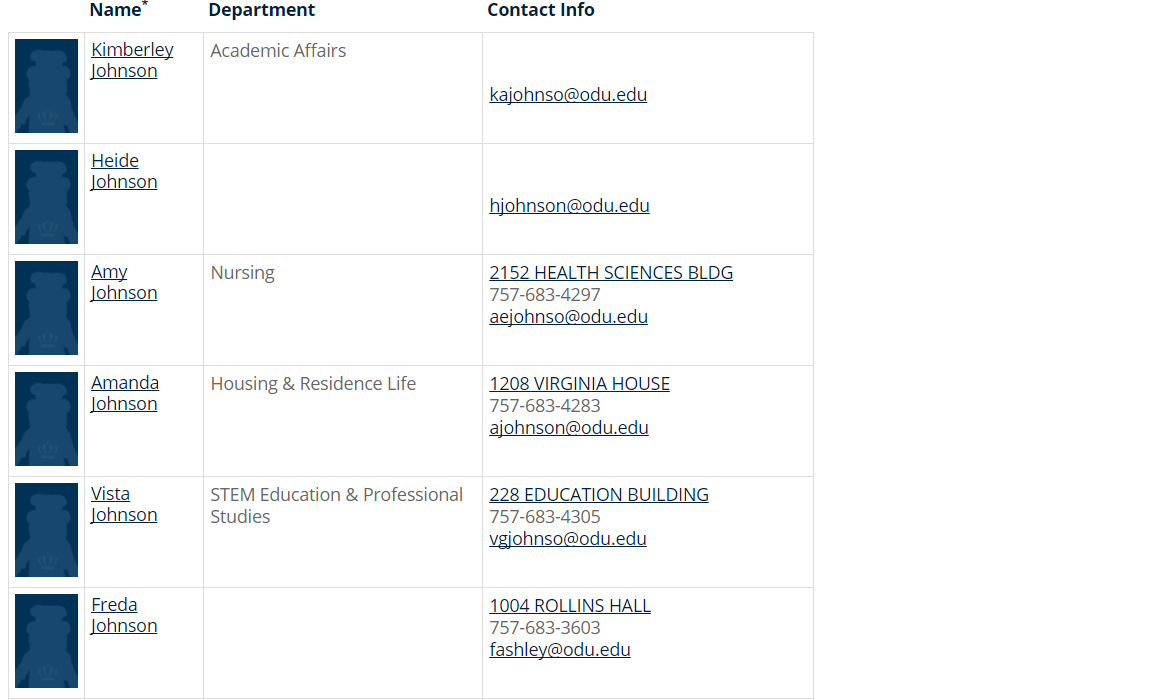
\includegraphics{odudirect.png}
  \captionof{figure} {student search result}
\end{center}

2. The second website is \url{https://www.amazon.com/}. This website also uses grep style of matching. It displays products by matching substrings. Amazon website ranks its products based on relevance . Figure 2 shows a search performed with ``shoe'' as a query and the result is a different shoe information based on grep style matching.

\begin{center}
  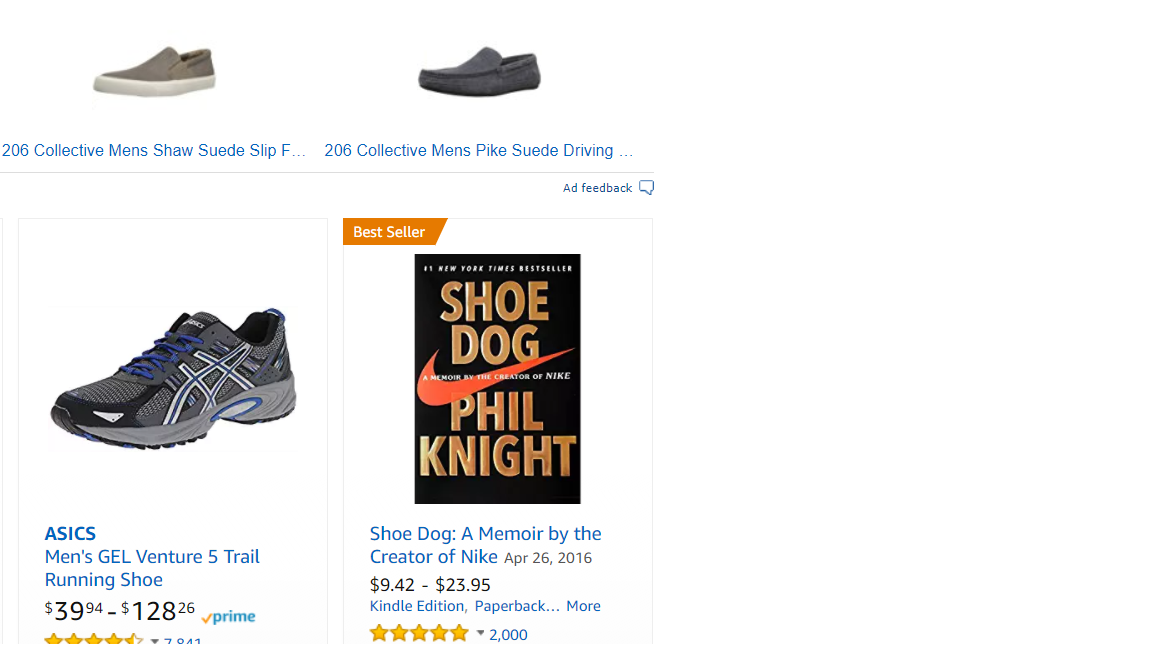
\includegraphics{amazon.png}
  \captionof{figure} {product search result}
\end{center}

3. The next website is \url{https://www.ebay.com/}. This site also uses grep style of matching and ranking is done based on category.\\

4. This kayak flight tracking website uses database style of matching. Here, the user searches with a flight number and this number is matched with the database table to retrieve relevant result. Because search is done with a number, there are no substrings to match. Figure 3 shows how flight is tracked by filling out the relevant field. Figure 3 gives the itenary of an American Airline flight with flight number 2192.

\begin{center}
  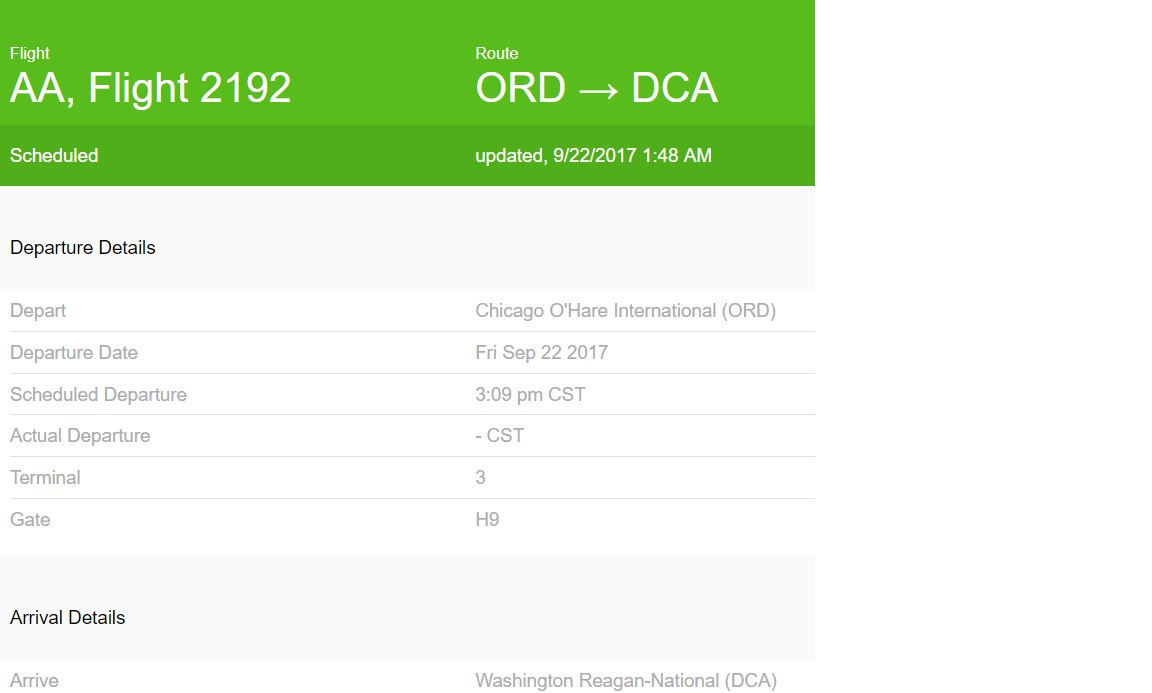
\includegraphics{flight.png}
  \captionof{figure} {flight tracker}
\end{center}

5. The last website is \url{http://www.ikea.com/us/en/}. This website uses grep style of matching and products are ranked based on relevance.








\end{homeworkProblem}


%----------------------------------------------------------------------------------------
% PROBLEM 5
%----------------------------------------------------------------------------------------
\begin{homeworkProblem}
Give a high-level outline of an algorithm that would use the DOM structure
to identify content information in a web page. In particular, describe heuristics
you would use to identify content and non-content elements of the structure.

\textbf{Solution 5:}\\

\textbf{Algorithm title:} Extract text content\\
\textbf{Input          : } HTML Page, P (Collection of HTML tags)\\
\textbf{Output         : }Text Content, P\\

\textbf{Description:} Using a predefined list L, of HTML tags, that are known to contain text for HTML pages, extract all tags of  kind same as L from the HTML page. Then if the tags do not contain elements inside, extract text enclosed by tags: $<tag>$ Text to extract $</tag>$. If the tag contain other tags inside, recursively visit every element in the tag until you reach the final tag, then extract text.\\
 \begin{verbatim}
 Given L,
    L = [div, span, p, h1, h2, h3, h4, title, a, strong, em, table, ]
    Procedure extractContent(HTML page P)
        G = extract all tags from P that is in L

        for tag t in G do
            if t has element then
                extractContent(t)
            else
                T.add(t.text content)
            endif

        endfor
    endProcedure
\end{verbatim}













\end{homeworkProblem}


\nocite{*}\clearpage
\bibliographystyle{plain}
\bibliography{A1Ref}


\end{document}

